\documentclass{article}
\usepackage{enumerate}
\usepackage{graphicx}
\usepackage{float}

\usepackage{amsmath}
\usepackage[margin=1in]{geometry}
\usepackage[parfill]{parskip}

\newcommand{\heading}[1]{\bigskip \textbf{#1}}

\title{Physics 112 Problem Set 1}
\author{Sahil Chinoy}
\date{September 8, 2017}

\begin{document}
\maketitle{}

\begin{enumerate}

\item

	\begin{enumerate}[(a)]

	\item

	$7^4 = 2401$

	\item

	$\frac{7!}{4!} = 840$

	\item

	$\frac{7!}{3!4!} = 140$

	\item

	$\frac{10!}{4!6!} = 210$

	\end{enumerate}

\item

	\begin{enumerate}[(a)]

	\item

	$P(5000) = \frac{10000!}{5000!5000!}(0.5)^{10000} = 0.00798$

	\item

	$P(5100)/P(5000) = \frac{5000!5000!}{5100!4900!} = 0.135$

	\item

	$P(6000)/P(5000) = \frac{5000!5000!}{6000!4000!} = 3.643 \times 10^{-88}$

	\item

	$P(6)/P(5) = \frac{5!5!}{6!4!} = 0.833$

	\end{enumerate}

\item

	\begin{enumerate}[(a)]

	\item

	The probability of a single sequence of $N$ trials with $n$ events occurring is $p^n(1-p)^{N-n}$, and there are ${N \choose n}$ sequences of length $N$ with $n$ events, so the total probability of $n$ events occurring is

	$$P(n) = \frac{N!}{n!(N-n)!} p^n(1-p)^{N-n}.$$

	\item

	With $\lambda = Np$, we have 

	\begin{align*}
	P(n) = \frac{N(n-1)(n-2)\ldots(N-n+1)}{n!} \left(\frac{\lambda}{N}\right)^n \left(1-\frac{\lambda}{N}\right)^{N-n} \\
	P(n) = \frac{N^n + \mathcal{O}(N^{n-1})}{n!} \left(\frac{\lambda}{N}\right)^n \left(1-\frac{\lambda}{N}\right)^{N-n}.
	\end{align*}

	For large $n$, this is approximately

	\begin{equation*}
	P(n) \approx \frac{\lambda^n}{n!} \left(1-\frac{\lambda}{N}\right)^{N-n}.
	\end{equation*}

	Take the limit as $n \to \infty$, and recall $\lim \limits_{x\to\infty} (1 + \frac{1}{x})^x = e$. Then

	\begin{equation*}
	P(n) \approx \frac{\lambda^n}{n!} e^{-\lambda}.
	\end{equation*}

	\end{enumerate}

\item

	\begin{enumerate}[(a)]

	\item

	\begin{align*}
	g(N,s) &= \frac{N!}{(N/2+s)! (N/2-s)!} \\
	g(N,s) &= \frac{\sqrt{2\pi N}N^N e^{-N}}{ \sqrt{2 \pi (N/2 + s)} \; (N/2+s)^{N/2+s} \; e^{-N/2-s} \sqrt{2 \pi (N/2 - s)} \; (N/2-s)^{N/2-s} \; e^{-N/2+s}} \\
	g(N,s) &= \frac{\sqrt{N}N^N}{\sqrt{2 \pi}} \frac{1}{N/2 \sqrt{(1+2s/N)(1-2s/N)}} \frac{1}{[N/2(1+2s/N)]^{N/2+s}} \frac{1}{[N/2(1-2s/N)]^{N/2-s}} \\
	g(N,s) &= \frac{\sqrt{2}N^N}{\sqrt{\pi N}} \frac{1}{(N/2)^N} \frac{1}{[(1 + 2s/N)(1 - 2s/N)]^{N/2}} \frac{1}{(1 + 2s/N)^{1/2 + s}} \frac{1}{(1 - 2s/N)^{1/2 - s}} \\
	g(N,s) &= 2^N \sqrt{\frac{2}{\pi N}} \left(1 - 4\frac{s^2}{N^2}\right)^{-N/2} \frac{(1-2s/N)^{s-1/2}}{(1+2s/N)^{s+1/2}}
	\end{align*}

	\item

	Call the expression from (a) $g_1(N,s)$ and the expression from (b) $g_2(N,s)$. Then 

	\begin{itemize}

		\item

		$g_1(10, 1) / g_2(10, 1) = 1.019$

		\item

		$g_1(1000,100) / g_2(1000,100) = 0.891$

		\item

		$g_1(1000, 10) / g_2(1000, 10) = 1.000.$

	\end{itemize}

	\item

	These are both approximations to the true multiplicity function, so it's expected that they give similar results. I expect the first function, $g_1$, to be more accurate, since it only used the assumption that $N \gg 1$, from the Stirling approximation. The function derived in class, $g_2$, also used this assumption, but added the additional assumption that $s \ll N$, from the Taylor expansion of $\ln(1 - 2s/N)$. This is why we see better agreement between the two functions for $g(1000, 10)$ than for $g(1000, 100)$, because the $s \ll N$ assumption is more accurate in the first case. The main limitation of the function in (a), then, is just the requirement that $N$ is large.

	\end{enumerate}

\item 

	\begin{enumerate}[(a)]

	\item

	\begin{align*}
	\langle m(s) \rangle &= \sum \limits_{m=-R}^R mP(m,s) \\
	&= \sum \limits_{m=-R}^R m \left[ \frac{R+m+1}{2R} P(m+1,s-1) + \frac{R-m+1}{2R} P(m-1, s-1) \right].
	\end{align*}

	Reindexing the sums,

	\begin{align*}
	\langle m(s) \rangle &= \sum \limits_{m'=-R+1}^{R+1} (m'-1) \left[ \frac{R+m'}{2R} P(m',s-1) \right] + \sum \limits_{m'=-R-1}^{R-1} (m'+1) \left[ \frac{R-m'}{2R} P(m', s-1) \right].
	\end{align*}

	We know $-R \leq m' \leq R$, since there are only $2R$ fleas, so the $m' = R+1$ and $m' = -R-1$ terms are unphysical, and we drop them. Furthermore, we can add the term indexed by $m=-R$ to the first sum and the term indexed by $m'=R$ to the second sum, since the value of these terms is zero. So

	\begin{align*}
	\langle m(s) \rangle &= \sum \limits_{m'=-R}^{R} (m'-1) \left[ \frac{R+m'}{2R} P(m',s-1) \right] + \sum \limits_{m'=-R}^{R} (m'+1) \left[ \frac{R-m'}{2R} P(m', s-1) \right] \\
	&= \left[ \frac{1}{2}\langle m(s-1) \rangle + \frac{1}{2R} \langle m^2(s-1) \rangle - \frac{1}{2} - \frac{1}{2R} \langle m(s-1) \rangle \right] + \\
	& \left[\frac{1}{2}\langle m(s-1) \rangle - \frac{1}{2R} \langle m^2(s-1) \rangle + \frac{1}{2} - \frac{1}{2R} \langle m(s-1) \rangle \right] \\
	&= \left(1 - \frac{1}{R} \right) \langle m(s-1) \rangle.
	\end{align*}

	\item 

	We will prove this by induction. At the beginning, the excess number of fleas on Rover is $n$, so $ 
	\langle m(0) \rangle = n = n(1 - 1/R)^0$. So the base case holds.

	Assume $\langle m(k) \rangle = n(1 - 1/R)^k$. Then from the recurrence relation in (a), $\langle m(k+1) \rangle = (1-1/R) \times n(1 - 1/R)^k = n(1 - 1/R)^{k+1}$.

	So, by induction, $\langle m(s) \rangle = n(1 - 1/R)^s$ for all integers $s \geq 0$.

	\item 

	\begin{figure}[H]
	\caption{$\langle m(s) \rangle$ for $R=10$}
	\centering
	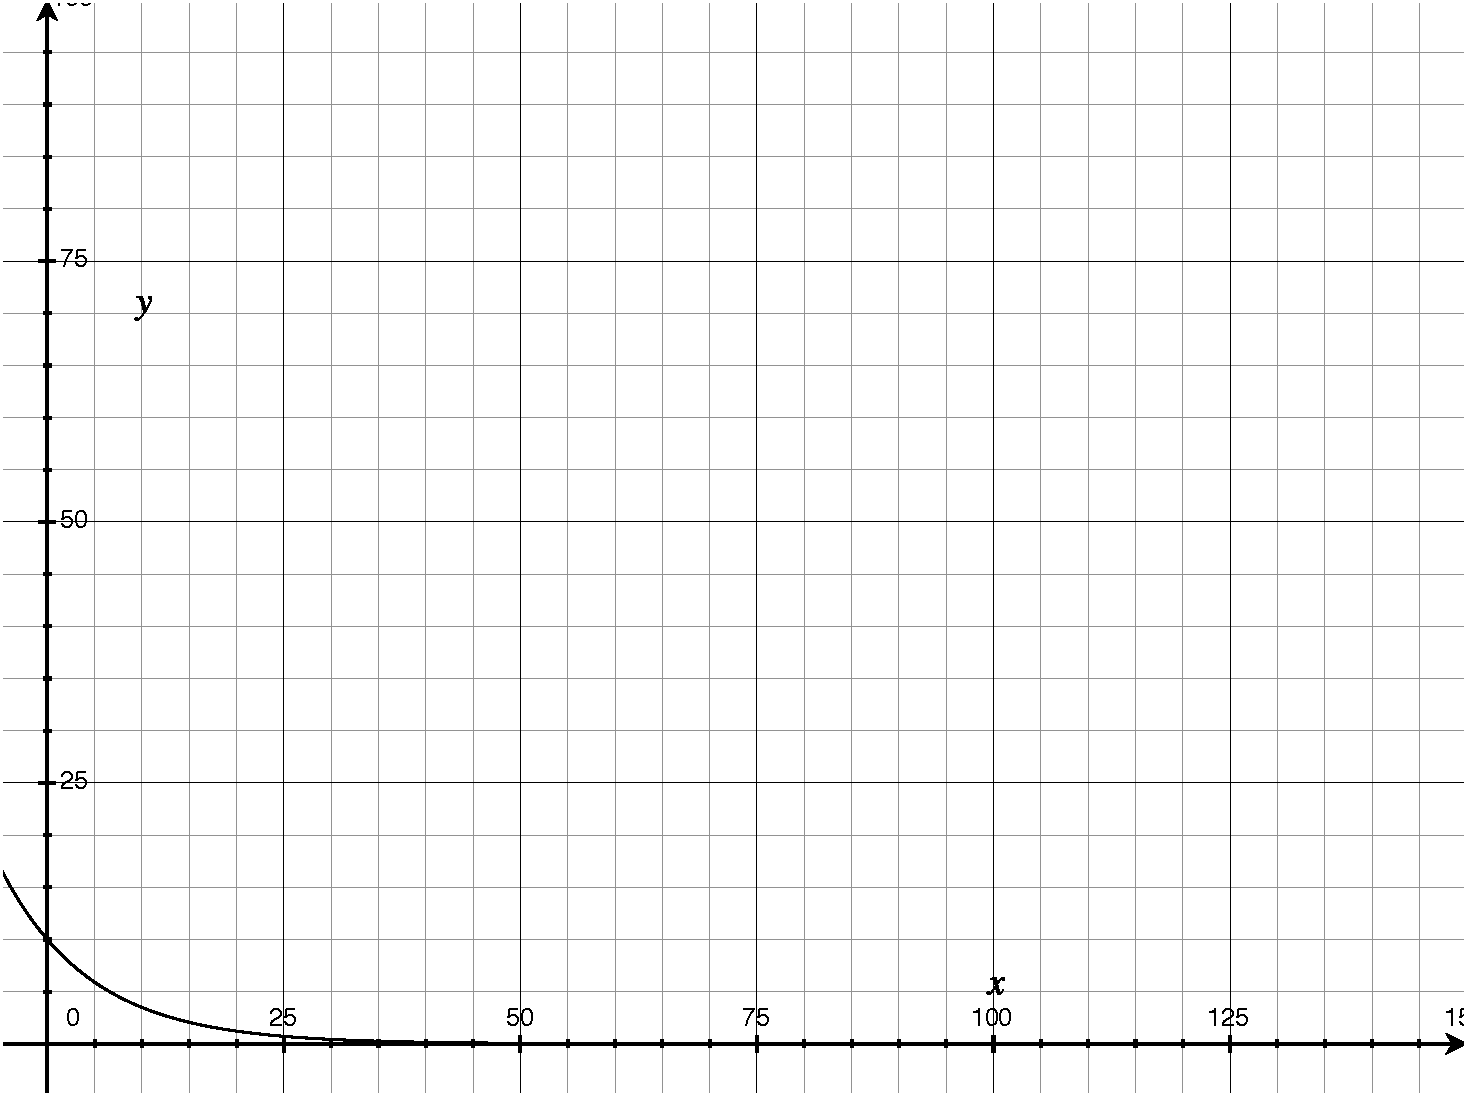
\includegraphics[width=10cm]{img/plot1}
	\end{figure}

	\begin{figure}[H]
	\caption{$\langle m(s) \rangle$ for $R=100$}
	\centering
	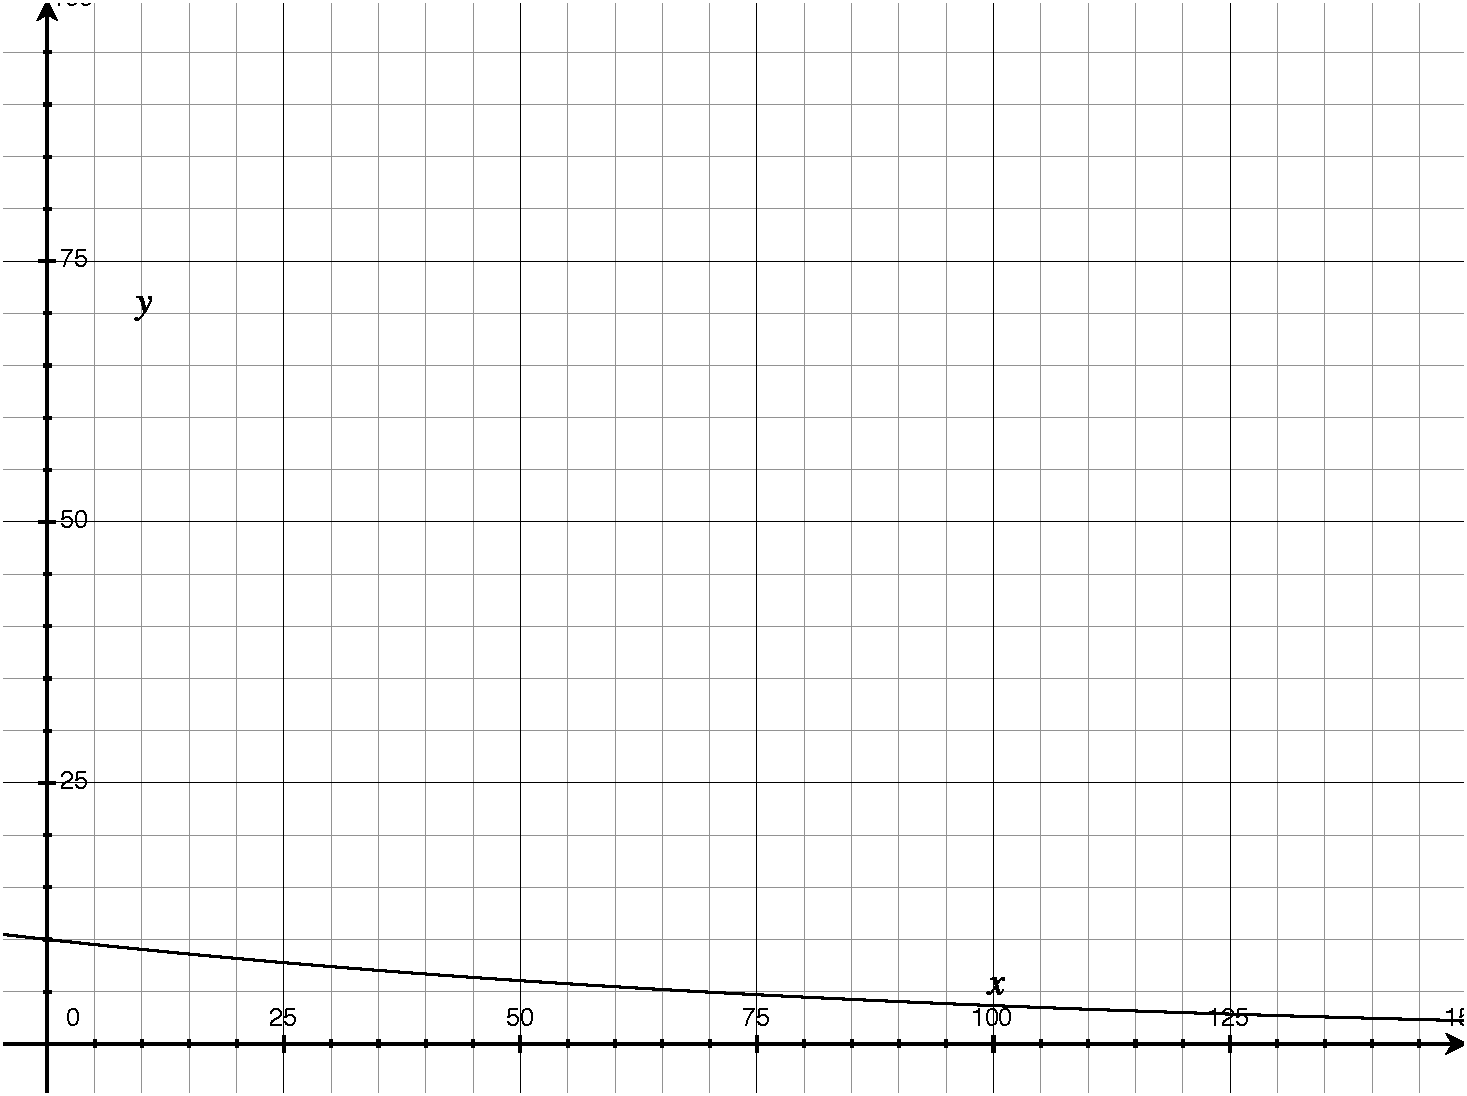
\includegraphics[width=10cm]{img/plot2}
	\end{figure}

	This behavior is roughly expected -- we expect the fleas to be equalized between the two dogs ($\langle m(s) \rangle \to 0$ as $s \to \infty$), and the more fleas they are (larger $R$), the longer this will take.

	\item

	For large $R$, $\langle m(s) \rangle = n \exp(s \ln(1 - 1/R)) \approx n \exp(-s/R)$. Making the analogy to RC circuits, the characteristic time scale of this exponential decay is $R$. That is, it takes about $R$ steps for the flea excess to fall off appreciably (to $1/e$). The larger the number of fleas, the longer it will take to reach equilibrium, and this relationship is roughly linear in $R$.

	\end{enumerate}

\item 

	\begin{enumerate}[(a)]

	\item

	The average path length is $10^{-5}$ m, and the projection of a path of this length in the $z$ direction is $10^{-5} \cos\theta$. So the average displacement in the $z$ direction, integrating over all solid angles, is 

	$$\langle z \rangle = \frac{1}{4\pi} \int\limits_0^\pi \int \limits_0^{2\pi} 10^{-5} \cos\theta \sin\theta \; d\phi d\theta = 0,$$

	as expected, since the particles are equally likely to travel in the $+z$ and $-z$ directions.

	\item

	The same argument applies, so

	$$\langle z^2 \rangle =  \frac{1}{4\pi} \int\limits_0^\pi \int \limits_0^{2\pi} (10^{-5} \cos\theta)^2 \sin\theta \; d\phi d\theta = 3.333 \times 10^{-11},$$

	thus $\sqrt{\langle z^2 \rangle} = 5.774 \times 10^{-6}$ m.

	\item 

	In 2 seconds, the ammonia molecules experience $N = 2 \times 10^7$ collisions. So we can think of the displacement in the $z$ direction as the sum of $2 \times 10^7$ independent random variables, each with mean $\langle z \rangle = 0$ and standard deviation $\sigma = \sqrt{\langle z^2 \rangle - \langle z \rangle ^2} = 5.774 \times 10^{-6}$ m.

	So, the average displacement after 2 seconds is $N \langle z \rangle = 0$. The standard deviation is $\sqrt{N}\sigma= \sqrt{2 \times 10^7} (5.774 \times 10^{-6}) = 0.0258$ m.

	\item

	The standard deviation after $t$ seconds is $\sqrt{t \times 10^7} (5.774 \times 10^{-6})$. When the standard deviation of $z$ is 6 m, approximately 32\% of the molecules are further than 6 m from the origin (assuming a Gaussian distribution, which is reasonable given the large number of molecules). This occurs at 

	$$t = \left( \frac{6}{\sqrt{10^7} (5.774 \times 10^{-6})} \right)^2 = 108000 \text{ s,}$$ or 300 hours.

	\end{enumerate}

\item

	\begin{enumerate}[(a)]

	\item

	$P = \left( \frac{1}{44} \right)^{100000}$, so $\log_{10}{P} = -10000\log_{10}44 = -164345$, thus $P = 10^{-164345}$.

	\item

	Typing $10$ keys per second, each monkey has typed $10^{18} \times 10 = 10^{19}$ keys since the beginning of the universe. Each key (approximately) represents the start of another $10^5$ character sequence. So the $10^{10}$ monkeys have had $10^{10} \times 10^{19} = 10^{29}$ opportunities to type Hamlet. The probability of any one random sequence resulting in Hamlet is $10^{-164345}$, from (a), so the probability that Hamlet has been typed is $10^{29} \times 10^{-164345} = 10^{-164316}$ (which is still extremely small).

	\end{enumerate}

\end{enumerate}

\end{document}